\chapter{Pengantar dan Model Matematika Big O}\label{ch:modul1}

\section{Pendahuluan}

\newthought{Algoritma} merupakan sebuah rangkaian proses komputasional yang mengkonversi satu atau beberapa masukan (\textit{input}) menjadi satu set keluaran (\textit{output}) jika memungkinkan. Untuk menyelesaikan permasalahan secara baik menggunakan algoritma, kita memerlukan tahapan analisis dan desain algoritma yang tepat dan benar. Tahapan desain akan menentukan bagaimana merancang algoritma kita sedangkan tahapan analisis akan menentukan seberapa banyak ruang (\textit{space}) dan seberapa lama waktu (\textit{time}) yang dibutuhkan algoritma tersebut. Secara umum langkah-langkah dalam penyelesaian masalah bisa dilihat di Gambar~\ref{fig:TahapanAnalisisDanDesain}.

\begin{figure}
    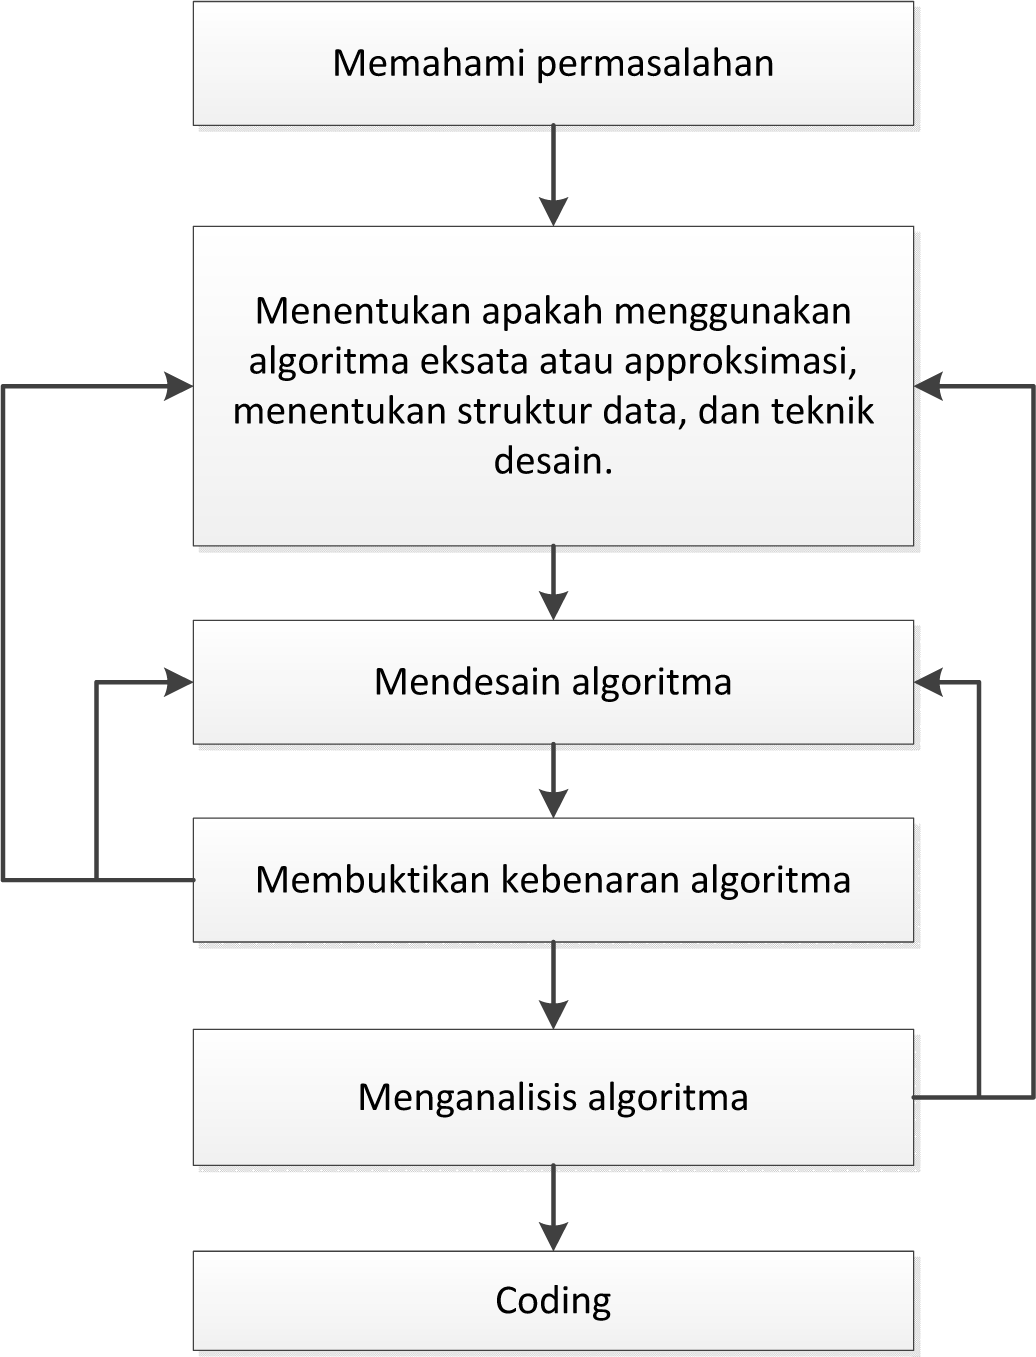
\includegraphics[scale=0.8]{fig/TahapanAnalisisDanDesain}
    \caption{Tahapan Analisis dan Desain Algoritma}
    \label{fig:TahapanAnalisisDanDesain}
\end{figure}

\subsection{Memahami permasalahan}
Memahami permasalahan merupakan langkah pertama dan merupakan langkah terpenting karena tanpa pemahaman yang baik langkah-langkah berikutnya tidak mungkin bisa terlaksana dengan baik. Pemahaman dilakukan dengan membaca deskripsi dari permasalahan secara baik. Apabila permasalahan tersebut merupakan permasalahan umum seperti misalnya masalah pengurutan, maka kita bisa menggunakan algoritma yang sudah ada untuk menyelesaikan. Jika tidak, maka kita harus mendesain dari awal algoritma tersebut.

Hal lain yang perlu diperhatikan baik-baik adalah masukan (\textit{input}) untuk permasalahan tersebut. Besarnya ukuran masukan menentukan algoritma yang akan kita gunakan. 

\subsection{Memilih antara penyelesaian permasalahan dengan pendekatan pasti (\textit{Exact}) atau approksimasi (\textit{Approximate})}
Yang dimaksud dengan pendekatan pasti adalah algoritma kita dijamin pasti bisa menemukan solusi dari permasalahan tersebut. Sedangkan pendekatan approksimasi, algoritma kita hanyalah memberikan hasil yang paling mendekati solusi sebenarnya. Kenapa perlu pendekatan approksimasi? Karena terkadang pendekatan pasti tidak bisa menemukan solusi dari permasalahan yang ada (bisa disebabkan karena ruang permasalahan sangat besar sekali sehingga memerlukan waktu yang sangat lama untuk menemukan solusinya).
 

\subsection{Menentukan struktur data}
Beberapa algoritma memerlukan struktur data tertentu seperti contohnya \textit{graph}. Struktur data yang tepat bisa memudahkan dan meningkatkan efisiensi waktu dan ruang dari implementasi sebuah algoritma tertentu. 

\subsection{Menentukan teknik desain algoritma}
Bagaimana jika permasalahan yang akan kita selesaikan tidak memiliki algoritma umum yang cocok untuk kita gunakan langsung? Maka kita harus mendesain algoritma tersebut dari awal. 

Untuk mendesain sebuah algoritma kita memerlukan teknik desain algoritma. Teknik desain algoritma merupakan sebuah pendekatan atau paradigma penyelesaian permasalahan yang bisa digunakan untuk berbagai jenis permasalahan yang ada. Salah satu contoh teknik desain algoritma adalah \textit{Divide and Conguer} dan \textit{Dynamic Programming}.

\subsection{Mendesain algoritma}
Jika kita sudah memahami permasalahan, menentukan struktur data dan teknik desain maka kita bisa melakukan desain algoritma. Desain algoritma bisa menggunakan bahasa perantara seperti \textit{pseudocode} atau \textit{flowchart}. Kita juga bisa langsung menggunakan bahasa pemrograman untuk mendesain algoritma. 

\subsection{Menentukan kebenaran dari algoritma}
Setelah sebuah algoritma selesai didesain, kita harus membuktikan kebenarannya atau dengan kata lain kita harus membuktikan bahwa algoritma kita memberikan solusi yang benar untuk semua masukan permasalahan dalam waktu yang terbatas. Ada beberapa cara untuk membuktikan kebenaran algoritma, salah satunya adalah menggunakan metode induksi matematika.

\subsection{Menganalisis algoritma}
Setelah mengetahui kebenaran dari sebuah algoritma maka langkah selanjutnya adalah mengetahui tingkat efisiensi ruang dan waktu dari algoritma tersebut. Efisiensi waktu menentukan seberapa cepat algoritma tersebut berjalan, sedangkan efisiensi ruang menentukan seberapa banyak memori yang diperlukan oleh algoritma tersebut. 

Untuk mengetahui seberapa effisien sebuah algoritma bisa dilakukan setelah menganalisis kompleksitas dari algoritma tersebut. Melakukan analisis algoritma berarti memprediksi berapa sumber daya (misalnya berapa lama waktu eksekusi atau berapa besar memori yang dibutuhkan) yang dibutuhkan oleh sebuah program ketika mengeksekusi algoritma tersebut. Pada umumnya, fokus analisis ditujukan pada waktu eksekusi dari algoritma tersebut walaupun tidak tertutup kemungkinan untuk menganalisi faktor lain.

Untuk mempermudah proses analisis, kita akan mengasumsikan bahwa algoritma kita akan berjalan di sebuah komputer dengan prossesor tunggal dan \textit{random-access machine} (RAM). Model RAM yang kita adopsi adalah model yang menjalankan algoritma secara baris per baris instruksi tanpa ada proses parallel. 

Instruksi yang diperbolehkan untuk dijalankan pada umumnya adalah instruksi penjumlahan `+', pengurangan `-', perkalian `*', pembagian `/', modulus `\%', pembulatan atas `$\left\lceil\  \right\rceil$', dan pembulatan bawah `$\left\lfloor\ \right\rfloor$', penyimpanan/pengeluaran/duplikat data ke variabel (mis: $a = 5$ dan $a = b$), dan kontrol (IF, FOR, WHILE, RETURN dan sebagainya). Semua dari instruksi tersebut menggunakan waktu secara konstan (artinya memiliki nilai yang sama apapun kondisinya, kecuali disebutkan secara eksplisit).

Untuk setiap analisis, ada tiga jenis kasus yang mungkin terjadi, yaitu: kasus terbaik, kasus terburuk dan kasus rata-rata. Dalam pengurutan, kasus terbaik adalah ketika kita hendak mengurutkan rangkaian bilangan yang sudah terurut. Sedangkan kasus terburuk adalah ketika kita hendak mengurutkan rangkaian bilang yang terurut terbalik. Untuk kasus-kasus rangkaian bilang acak lainnya, kita gunakan kasus rata-rata.

\section{Pengenalan Kompleksitas Algoritma}
Hasil dari analisis biasanya berupa kompleksitas algoritma. Kita ambil contoh \textit{Insertion Sort}, dimana waktu yang diperlukan bagi \textit{Insertion Sort} untuk menyelesaikan proses pengurutannya tergantung pada jumlah masukan. Dengan kata lain, semakin besar jumlah masukan, semakin lama waktu yang diperlukan. Untuk dua masukan dengan jumlah yang sama, \textit{Insertion Sort} bisa memakan waktu yang berbeda tergantung dari seberapa terurutnya mereka. Dari sini, kita bisa mengambil kesimpulan bahwa, waktu yang diperlukan berkembang sesuai dengan ukuran dari masukan.

Besar masukan sebuah algoritma sangat tergantung terhadap permasalahan yang sedang dihadapi. Sebagai contohnya, jika berbicara mengenai permasalahan pengurutan maka besar masukan berupa berapa banyak bilangan dalam sebuah \textit{array} atau \textit{array size}. Untuk permasalahan lain seperti misalnya permasalahan pencarian rute terpendek dimana masukannya adalah berupa \textit{graph}, maka yang menjadi besar masukannya adalah jumlah \textit{vertice} dan \textit{edge} dari \textit{graph} tersebut. 

\section{Kompleksitas Algoritma}
Algoritma yang berbeda tentu saja memiliki langkah-langkah yang berbeda. Sehingga, ada algoritma yang lebih cepat dibandingkan algoritma yang lain. Dan ada pula algoritma yang lebih hemat dalam penggunaan memori. Algoritma yang baik adalah algoritma yang dapat menyelesaikan masalah  sekaligus efisien dalam pemakaian waktu dan ruang. Istilah yang digunakan untuk mengukur hal tersebut adalah \textbf{kompleksitas algoritma}. Maka, terdapat 2 jenis kompleksitas algoritma, yakni:

\begin{itemize}
    \item kompleksitas waktu ($T(n)$), dan
    \item kompleksitas ruang ($S(n)$).
\end{itemize}

Tentu diperlukan sebuah metode untuk mengukur seberapa cepat sebuah algoritma atau seberapa hemat pemakaian ruang memori dari algoritma tersebut. Menganalisis sebuah algoritma mencakup menganalisis kompleksitas algoritma. Meskipun terdapat 2 jenis kompleksitas, pada kuliah analisis dan desain algoritma ini yang lebih difokuskan adalah analisis kecepatan algoritma tersebut, atau kompleksitas waktunya ($T(n)$).

Cepat atau lambatnya sebuah algoritma tidak dihitung menggunakan satuan waktu yang umum digunakan dalam kehidupan, seperti detik, menit, ataupun jam. Alasannya karena kecepatan proses sebuah algoritma yang sudah diimplementasikan ke dalam program komputer bergantung pada banyak faktor, seperti prosessor, sistem operasi, \textit{compiler} yang digunakan, dan faktor lain. Menghitung kompleksitas waktu sebuah algoritma adalah \textbf{menghitung jumlah langkah yang ditempuh, serta perubahan jumlah langkah saat ukuran input berubah}. Jadi, tidak akan ada hubungannya dengan performa komputer atau kompiler yang digunakan sebagai media implementasi algoritma tersebut.

Pada banyak algoritma, jumlah langkah yang ditempuh sangat bergantung kepada ukuran dari masukan algoritma tersebut. Besar masukan sebuah algoritma sendiri sangat tergantung terhadap permasalahan yang sedang dihadapi. Sebagai contohnya, jika berbicara mengenai permasalahan pengurutan maka besar masukan berupa berapa banyak bilangan dalam sebuah \textit{array} (\textit{array size}). Untuk permasalahan lain seperti misalnya permasalahan pencarian rute terpendek dimana masukannya adalah berupa \textit{graph} (akan dijelaskan di mata kuliah struktur data), maka yang menjadi besar masukannya adalah jumlah \textit{vertice} dan \textit{edge} dari \textit{graph} tersebut. 


Banyaknya varian masukan serta cara perhitungan ukuran masukan yang berbeda-beda ini pada akhirnya menyebabkan perhitungan kompleksitas waktu algoritma memerlukan sebuah notasi khusus: \textbf{notasi asimtotik}.

\section{Notasi Asimtotik}

Sebagaimana dijelaskan pada sub-bagian di atas, untuk mengukur kompleksitas waktu algoritma tidak digunakan satuan waktu yang umum. Maka, dibutuhkan sebuah notasi khusus. Notasi matematis yang digunakan disebut \textbf{notasi asimtotik}. Notasi asimtotik digunakan untuk melihat seberapa efisien performa sebuah algoritma bila dibandingkan dengan algoritma yang lain. 

Terdapat beberapa jenis notasi asimtotik dalam bidang ilmu matematika yang digunakan dalam pengukuran kompleksitas algoritma. 3 contoh jenis notasi asimtotik adalah:

\begin{enumerate}
    \item O (Big-O)
    \item $\Omega$ (Big-Omega)
    \item $\Theta$ (Big-Theta)
\end{enumerate}

Dalam modul ini tidak akan dijelaskan secara terperinci bagaimana menggunakan masing-masing notasi. Namun, yang akan dijelaskan adalah bagaimana kompleksitas waktu sebuah algoritma dapat ditemukan dengan menggunakan notasi tersebut.

Notasi yang paling umum digunakan adalah O (Big-O). Alasannya adalah karena notasi tersebut digunakan untuk menggambarkan batas atas (\textit{upper limit}) dari sebuah fungsi ketika masukan untuk fungsi tersebut meningkat (\textit{increase}). Alhasil, Big-O sangat cocok untuk memperlihatkan \textit{worst case} dari sebuah algoritma. Apa yang dimaksud dengan worst case akan dijelaskan pada salah satu sub-bagian dari modul ini.

Contoh notasi Big-O: Algoritma Bubble Sort memiliki kompleksitas $T(n) = O(n^2)$. Artinya: algoritma Bubble Sort memiliki kompleksitas waktu $n^2$. 

\section{Mengukur Kompleksitas Algoritma Menggunakan Big-O}

Secara umum pengukuran kompleksitas algoritma dilakukan dengan melakukan perhitungan terhadap \textbf{pertumbuhan} jumlah langkah yang diperlukan untuk menyelesaikan sebuah algoritma. Biasanya langkah-langkah ini dihitung dengan cukup gamblang, yaitu dengan langsung menghitung berapa kali satu baris algoritma dijalankan.

Walaupun kedengarannya cukup mudah, perlu dicatat juga bahwa yang dijelaskan sebelumnya hanyalah cara menghitung kompleksitas algoritma non rekursif. Perhitungan kompleksitas algoritma non-rekursif tidak persis dengan algoritma rekursif. Untuk memulai pembahasan, kita akan membahas perhitungan kompleksitas pada algoritma non-rekursif terlebih dahulu. Kita baru akan membahas cara perhitungan kompleksitas algoritma rekursif pada bab berikutnya. Begitupun, dasar perhitungan kompleksitas adalah sama: menggunakan fungsi matematis dan aturan dasar penjumlahan.

Pada setiap modul, seraya berbagai teknik desain algoritma akan dibahas, juga akan diperlihatkan bagaimana menghitung kompleksitas algoritmanya. 

Secara umum, langkah-langkah untuk mengukur kompleksitas algoritma non-rekursif adalah sebagai berikut:

\begin{enumerate}
    \item Mengidentifikasi operasi dasar.
    \item Menentukan ukuran input.
    \item Memeriksa apakah pertumbuhan operasi dasar hanya bergantung pada ukuran input. Jika ya, maka tidak ada \textit{worst case} ataupun \textit{best case}. Namun jika terdapat faktor lain, maka perhitungan \textit{worst case} dibedakan dengan \textit{best case}.
    \item Menghitung derajat pertumbuhan langkah operasi dasar terhadap perubahan ukuran input dengan menggunakan fungsi matematika.
\end{enumerate}

Beberapa rumus matematika yang dapat digunakan untuk menunjang langkah keempat yaitu:

\begin{equation}\label{eq:common-1}
    \sum\limits_{i=l}^u 1 = 1 + 1 + 1 + 1 + \ldots = u - l + 1
\end{equation}

\begin{equation}\label{eq:common-2}
    \sum\limits_{i=1}^n 1 = n
\end{equation}

\begin{equation}\label{eq:common-3}
    \sum\limits_{i=1}^n i = 1 + 2 + \cdots + n = \frac{n(n + 1)}{2} \approx \frac{1}{2}n^2
\end{equation}

\begin{equation}\label{eq:common-4}
    \sum\limits_{i=1}^n i^2 = 1^2 + 2^2 + \cdots + n^2 = \frac{n(n + 1)(2n + 1)}{6} \approx \frac{1}{3}n^3
\end{equation}

\begin{equation}\label{eq:common-5}
    \sum\limits_{i=1}^n i^k = 1^k + 2^k + \cdots + n^k \approx \frac{1}{k + 1}n^{k+1}
\end{equation}

\begin{equation}\label{eq:common-6}
    \sum\limits_{i=0}^n a^i = 1 + a + \cdots + a^n = \frac{a^{n + 1} - 1}{a - 1}(a \neq 1)
\end{equation}

\begin{equation}\label{eq:common-7}
    \sum\limits_{i=0}^n 2^i = 2^{n + 1} - 1
\end{equation}

\begin{equation}\label{eq:common-8}
    \sum\limits_{i=1}^n i \times 2^i = 1 \times 2^1 + 2 \times 2^2 + \cdots + n \times 2^n \approx \frac{1}{3}n^3
\end{equation}

\begin{equation}\label{eq:common-9}
    \sum\limits_{i=l}^u ca_i = c \sum\limits_{i=l}^u a_i
\end{equation}

\begin{equation}\label{eq:common-10}
    \sum\limits_{i=l}^u (a_i \pm b_i) = \sum\limits_{i=l}{u} a_i \pm \sum\limits_{i=l}{u} b_i
\end{equation}

Biasanya kita akan mengubah deret langkah yang didapatkan melalui hasil perhitungan kompleksitas ke dalam bentuk yang lebih sederhana, dengan menggunakan fungsi-fungsi matematika di atas.

Untuk memperjelas, kita akan langsung mencoba melakukan perhitungan kompleksitas terhadap sebuah algoritma sederhana. Misalkan kita memiliki algoritma untuk menghitung nilai maksimum di dalam sebuah \textit{array} seperti berikut:

\lstinputlisting[language=Python, 
                 label={algo:maxelem},
                 caption=Maximum Element
                ]
                {code/1-max-element.py}

\FloatBarrier

Langkah-langkah yang dijalankan untuk menghitung kompleksitas yaitu:

\begin{enumerate}
    \item \textbf{Mengidentifikasi operasi dasar.} Operasi dasar adalah perbandingan antara \textbf{maximum} dan \textbf{arr[i]} pada baris ke 7, karena operasi ini merupakan operasi yang paling sering dilakukan yang merupakan logika dasar algoritma tersebut untuk memecahkan masalah.
    \item \textbf{Menentukan ukuran input.} Ukuran input adalah \textbf{arr\_len}, yang merupakan besar / panjang dari array atau list \textbf{arr}. \textbf{arr\_len} menjadi ukuran input karena berpengaruh terhadap banyaknya operasi dasar dilakukan.
    \item \textbf{Memeriksa apakah pertumbuhan operasi dasar hanya bergantung pada ukuran input.} Untuk algoritma pada listing~\ref{algo:maxelem}, \textbf{arr\_len} merupakan satu-satunya penentu banyaknya operasi dasar dilakukan, sehingga dalam perhitungan kompleksitas tidak diikutsertakan analisis \textit{worst case}, \textit{best case}, maupun \textit{average case}.
    \item \textbf{Menghitung derajat pertumbuhan langkah operasi dasar terhadap perubahan ukuran input dengan menggunakan fungsi matematika.} 
\end{enumerate}

Langkah keempat memerlukan perhitungan yang lebih mendetail. Derajat pertumbuhan yang dimaksud adalah seberapa besar pengaruh sebagian kode terhadap jumlah langkah keseluruhan dari sebuah algoritma. Pada algoritma dalam lsiting~\ref{algo:maxelem}, bagian yang mempengaruhi adalah bagian perulangan, tepatnya pada bagian yang diwarnai dalam listing~\ref{algo:maxelem-highlighted}.

\lstinputlisting[language=Python, 
                 caption=Perulangan pada Maximum Element, 
                 label={algo:maxelem-highlighted},
                 linebackgroundcolor={\ifnum\value{lstnumber}>5\ifnum\value{lstnumber}<11\color{codehighlight}\fi\fi}
                ]
                {code/1-max-element.py}

\FloatBarrier

Penjelasan: Perulangan merupakan deret, sehingga perulangan yang terpola dengan baik dapat digantikan ke dalam fungsi matematis berikut:

\begin{equation}\label{eq:maxelem-loop}
    T(n) = \sum\limits_{i=0}^{n-1} 1
\end{equation}

Isi dari sigma berisi 1 karena: \textbf{dalam setiap perulangan terdapat 1 kali operasi dasar yang dilakukan}. Selanjutnya, kita akan menggunakan rumus matematika~\ref{eq:common-1} pada fungsi~\ref{eq:maxelem-loop}:

\begin{equation}\label{eq:maxelem-loop-2}
T(n) = n - 1 + 1 = n
\end{equation}

Selanjutnya hasil akhir pada persamaan~\ref{eq:maxelem-loop-2} diubah ke dalam notasi asimtotik sesuai dengan aturan notasi seperti berikut:

$$
T(n) = O(n)
$$

Alhasil, algoritma di atas memiliki kompleksitas $O(n)$, atau sering disebut dengan kompleksitas linear.

\section{Kriteria Efisiensi umum}

Sebelum membahas lebih banyak contoh perhitungan kompleksitas lagi, kita akan terlebih dahulu melihat berbagai kriteria efisiensi algoritma yang ada. Terdapat beberapa kriteria efisiensi umum, yaitu:

\begin{enumerate}
    \item \textbf{$O (1)$: Kompleksitas Konstan.} Merupakan kriteria di mana ukuran input sama sekali tidak berpengaruh pada jumlah langkah sebuah algoritma. Kompleksitas ini merupakan jenis yang paling efisien / cepat.
        
    \begin{figure}
        \centering
        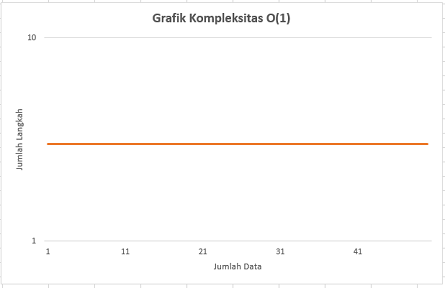
\includegraphics[width=\textwidth]{fig/ConstantGrowth}
        \caption{Grafik Pertumbuhan Konstan}
        \label{fig:ConstantGrowth}
    \end{figure}

    \FloatBarrier

    \item \textbf{$O (\log n)$: Kompleksitas Logaritmik.} Merupakan kompleksitas di mana perubahan / peningkatan besar dari ukuran input hanya memberikan sedikit sekali pengaruh terhadap pertumbuhan jumlah langkah. Algoritma yang memiliki kompleksitas logaritmik sering dijumpai pada algoritma yang dibuat dengan teknik divide \& conquer yang akan dibahas pada salah satu modul.

    \begin{figure}
        \centering
        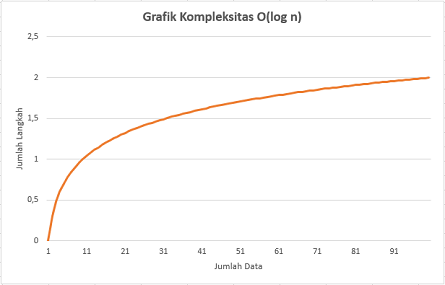
\includegraphics[width=\textwidth]{fig/LogarithmicGrowth}
        \caption{Grafik Pertumbuhan Logaritmik}
        \label{fig:LogarithmicGrowth}
    \end{figure}

    \FloatBarrier

    \item \textbf{$O (n)$: Linear.} Merupakan kompleksitas algoritma di mana pertumbuhan ukuran input sebanding dengan pertumbuhan jumlah langkah. Algoritma dengan kompleksitas linear dipandang sebagai algoritma yang cepat / efisien, meskipun itu juga bergantung pada permasalahan apa yang diselesaikan oleh sebuah algoritma.

    \begin{figure}
        \centering
        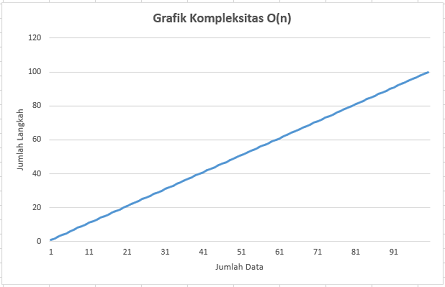
\includegraphics[width=\textwidth]{fig/LinearGrowth}
        \caption{Grafik Pertumbuhan Linear}
        \label{fig:LinearGrowth}
    \end{figure}

    \FloatBarrier

    \item \textbf{$O (n \log n)$.} Kompleksitas ini belum memiliki nama khusus. Jenis kompleksitas ini juga sering dijumpai pada algoritma yang berbasis teknik divide \& conquer. Hanya saja, pada kompleksitas jenis ini, perubahan jumlah langkah sedikit lebih besar daripada kompleksitas linear.

    \begin{figure}
        \centering
        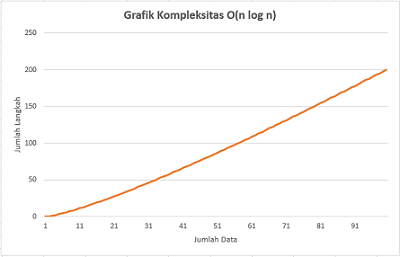
\includegraphics[width=\textwidth]{fig/NLogNGrowth}
        \caption{Grafik Pertumbuhan $n \log n$}
        \label{fig:NLogNGrowth}
    \end{figure}

    \FloatBarrier

    \item \textbf{$O (n^m)$: Kompleksitas Polinomial.} Merupakan jenis kompleksitas yang tinggi. $O (n^2)$ disebut dengan kompleksitas kuadratik. Merupakan jenis kompleksitas di mana sedikit perubahan pada ukuran input akan berpengaruh besar pada jumlah langkah.

    \begin{figure}
        \centering
        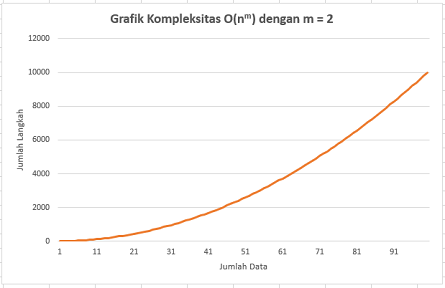
\includegraphics[width=\textwidth]{fig/ExponentialGrowth}
        \caption{Grafik Pertumbuhan Polinomial}
        \label{fig:ExponentialGrowth}
    \end{figure}

    \FloatBarrier

    \item \textbf{$O (n!)$: Kompleksitas faktorial.} Merupakan jenis kompleksitas yang sangat tinggi. Sedikit perubahan pada ukuran input akan berpengaruh sangat besar terhadap jumlah langkah. Kompleksitas ini sangat dihindari, namun untuk sebuah permasalahan komputasi yang sangat kompleks algoritma dengan kompleksitas yang tinggi juga sering digunakan.

    \begin{figure}
        \centering
        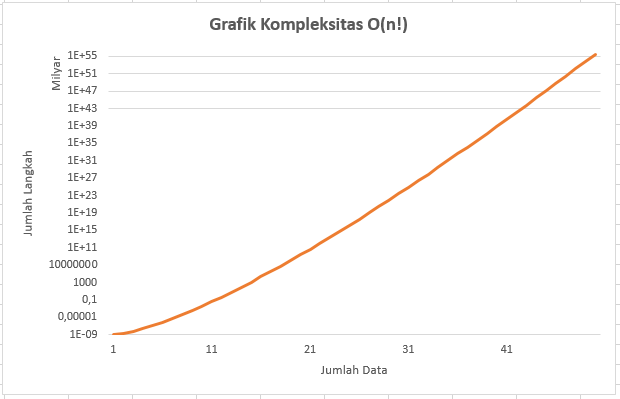
\includegraphics[width=\textwidth]{fig/FactorialGrowth}
        \caption{Grafik Pertumbuhan Faktorial}
        \label{fig:FactorialGrowth}
    \end{figure}

    \FloatBarrier
\end{enumerate}

Masing-masing kriteria efisiensi tersebut memiliki tingkat pertumbuhan yang berbeda-beda. Gambar~\ref{fig:allcomplexitycomparison} memperlihatkan perbandingan tingkat pertumbuhan dari masing-masing kriteria efisiensi. Perhatikan bagaimana $O(1)$ tak lagi terlihat di dalam gambar~\ref{fig:allcomplexitycomparison} karena nilainya yang sangat kecil (paling efisien).

\begin{figure}
    \centering
    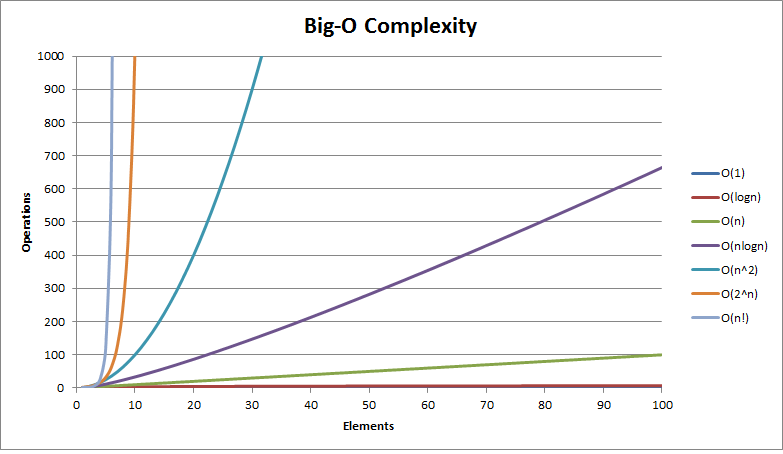
\includegraphics[width=\textwidth]{fig/AllComplexityComparison}
    \caption{Perbandingan Tingkat Pertumbuhan Seluruh Kriteria Efisiensi}
    \label{fig:allcomplexitycomparison}
\end{figure}

    \FloatBarrier

\section{Worst Case, Average Case, dan Best Case}

Dalam pengukuran kompleksitas algoritma, terdapat \textit{worst case}, \textit{average case}, dan \textit{best case}.

\begin{enumerate}
    \item Best case / kasus terbaik: merupakan kondisi di mana algoritma akan bekerja dengan kompleksitas paling rendah untuk ukuran input yang sama. Biasanya kasus \textit{best case} terjadi ketika algoritma menerima kondisi masukan yang optimal. Misalnya pada algoritma pengurutan, kondisi \textit{best case} dapat tercapai ketika kita memberikan masukan \textit{array} yang telah terurut. Hal ini memastikan algoritma akan berjalan dengan jumlah langkah minimal.
    \item Worst case / kasus terburuk: merupakan kebalikan dari kasus terbaik, di mana algoritma akan bekerja dengan kompleksitas tertinggi untuk ukuran input yang sama. Bertolak belakang dengan \textit{best case}, \textit{worst case} ditemukan ketika masukan sangat tidak optimal, sehingga algoritma harus berjalan dengan jumlah langkah maksimal.
    \item Average case / kasus rata-rata: merupakan kondisi yang paling sering terjadi untuk sebuah permasalahan.
\end{enumerate}

Pada prakteknya, pengukuran yang paling sering kita gunakan adalah pengukuran \textit{worst case} dan \textit{average case}. Begitupun, pengukuran \textit{best case} memiliki kegunaannya sendiri, misalkan pada kasus di mana kita mengetahui dengan persis seluruh masukan yang akan diterima.

\section{Contoh Kasus: Analisis Faktorial Iteratif}

Misalkan kita memiliki sebuah algoritma untuk menghitung faktorial dari sebuah bilangan sebagai berikut:

\lstinputlisting[language=Python, 
                 label={algo:faktorial},
                 caption=Algoritma Perhitungan Faktorial,
                 float
                ]
                {code/4-faktorial.py}

Kita dapat menghitung jumlah langkah yang harus dijalankan oleh algoritma~\ref{algo:faktorial} seperti berikut:

\begin{figure}%
    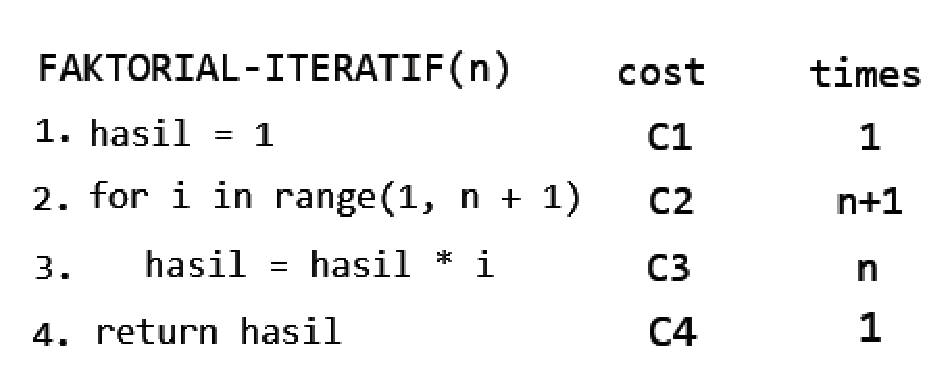
\includegraphics[scale=0.5]{fig/faktorialAnalysis}%
    \caption{Analisis Faktorial}%
    \label{fig:analisis-faktorial}%
\end{figure}

\FloatBarrier

Untuk mempermudah perhitungan, biasanya setiap langkah dianggap menghabiskan waktu yang konstan yaitu konstanta $c_i$ dimana $i$ menandakan baris keberapa dari \textit{pseudocode} algoritma tersebut. Nilai dari $c_i$ sendiri tidaklah penting, yang penting adalah berapa kali konstanta $c_i$ itu dieksekusi. Dari Gambar \ref{fig:analisis-faktorial}, setiap langkah (baris) memiliki biaya (\textit{cost}) eksekusi. 
Biaya eksekusi tersebut dilambangkan dengan besarnya konstanta $c_i$ yang dikalikan banyaknya konstanta tersebut dieksekusi yaitu $n$, dengan kata lain lamanya waktu yang dibutuhkan untuk mengeksekusi setiap langkah adalah $c_{i}\times{}n$ atau disingkat $c_{i}n$

Penjelasan lebih detil dari Gambar \ref{fig:analisis-faktorial} adalah sebagai berikut.

\begin{enumerate}
	\item Baris 1: Memiliki biaya sebesar $c_1$ dimana biaya tersebut akan diulang sebesar $1$ kali.  
	\item Baris 2: Memiliki biaya sebesar $c_2$ dimana biaya tersebut akan diulang sebesar $n+1$ kali. Pengulangan sebesar $n+1$ kali dikarenakan adanya sebuah looping ``\textbf{for i in range(1, n + 1)}''. Looping \textbf{for} akan dieksekusi oleh komputer sebanyak $n+1$ kali. Untuk mempermudah perhitungan maka kita misalkan $n$ bernilai 5, maka baris 2 akan diulang sebanyak 6 kali (1,2,3,4 dan 5 bernilai $True$ dan 1 kali terakhir bernilai $False$) atau $n$+1 kali.
	\item Baris 3: Memiliki biaya $c_{3}$. Ketiga baris tersebut masing-masing diulang sebanyak $n$ kali. Kenapa $n$ kali? Karena semua baris di dalam \textit{looping} \textbf{for} hanya diulang untuk setiap \textbf{for} yang bernilai $True$.
	\item Baris 4: Memiliki biaya 1 dan hanya berjalan 1 kali, yaitu ketika fungsi mengembalikan nilai ke pemanggilnya.
\end{enumerate}

Total waktu eksekusi dari Algoritma Faktorial Iteratif dilambangkan dengan $T(n)$ dimana:
\begin{equation}\label{eq:eksekusi-faktorial}
    \begin{aligned}
        T(n) &= c_{1} + c_{2}(n+1) + c_{3}n + c_{4}    \\ 
             &= c_{1} + c_{2}n + c_{2} + c_{3}n + c{4} \\
             &= (c_{2}+c_{3})n + (c_{1}+c_{2}+1)
    \end{aligned} 
\end{equation}

Persamaan \ref{eq:eksekusi-faktorial} bisa disederhanakan menjadi 

\begin{equation}\label{eq:faktorial-final}
    T(n) = an + b 
\end{equation}


Dari persamaan \ref{eq:faktorial-final} yaitu $an$ + $b$, terdapat dua konstan ($a$, dan $b$) yang besarnya tergantung pada $c_i$. Untuk membuat lebih sederhana, kita bisa membuat abstraksi yang lebih sederhana yaitu dengan hanya memperhatikan laju pertumbuhan fungsi (\textit{order of growth}). Untuk itu kita cukup hanya perlu memperhatikan order tertinggi dari fungsi yaitu $an$ karena order yang lebih rendah lajut pertumbuhannya tidak begitu signifikan untuk nilai $n$ yang besar.

Dengan perhitungan dan analisa di atas, dapat kita simpulkan bahwa algoritma faktorial di atas memiliki kompleksitas $O(n)$.

\section{Contoh Kasus: Analisis \textit{Bubble Sort}}

Sebagai contoh selanjutnya, kita akan melakukan analisa terhadap algoritma pengurutan nilai yang sangat sederhana dan naif: \textit{Bubble Sort}. Sebelum mulai melihat dan menganalisa algoritma, terlebih dahulu kita akan menentukan aturan dan batasan dari contoh kasus yang kita gunakan dalam modul ini.

Untuk mempermudah proses analisis, kita akan mengasumsikan bahwa algoritma yang diuji berjalan di sebuah komputer dengan prossesor tunggal dan \textit{random-access machine} (RAM). Model RAM yang kita adopsi adalah model yang menjalankan algoritma secara baris per baris instruksi tanpa ada proses parallel. 

Instruksi yang diperbolehkan untuk dijalankan pada umumnya adalah instruksi penjumlahan `+', pengurangan `-', perkalian `*', pembagian `/', modulus `\%', pembulatan atas `$\left\lceil\  \right\rceil$', dan pembulatan bawah `$\left\lfloor\ \right\rfloor$', penyimpanan/pengeluaran/duplikat data ke variabel (mis: $a = 5$ dan $a = b$), dan kontrol (IF, FOR, WHILE, RETURN dan sebagainya). Semua dari instruksi tersebut menggunakan waktu secara konstan (artinya memiliki nilai yang sama apapun kondisinya, kecuali disebutkan secara eksplisit).

Untuk setiap analisis, ada tiga jenis kasus yang mungkin terjadi, yaitu: kasus terbaik, kasus terburuk dan kasus rata-rata. Dalam pengurutan, kasus terbaik adalah ketika kita hendak mengurutkan rangkaian bilangan yang sudah terurut. Sedangkan kasus terburuk adalah ketika kita hendak mengurutkan rangkaian bilang yang terurut terbalik. Untuk kasus-kasus rangkaian bilang acak lainnya, kita gunakan kasus rata-rata.

Setelah aturan ditetapkan dengan benar, kita akan langsung mencoba melakukan analisa terhadap algoritma pertama, yaitu \textit{Bubble Sort}. Perhatikan implementasi algoritma \textit{Bubble Sort} berikut:

\lstinputlisting[language=Python, 
                 label={algo:bubble},
                 caption=Algoritma Bubble Sort,
                 float
                ]
                {code/2-bubble-sort.py}

Sebelum menganalisis Algoritma \ref{algo:bubble} ada dua hal penting yang harus dipahami terlebih dahulu: besar masukan (\textit{input size}) dan waktu eksekusi (\textit{running time}). 

\begin{figure}[htbp]%
	\includegraphics[scale=0.6]{fig/BubbleAnalysis}%
	\caption{Analisis \textit{Bubble Sort}}%
	\label{fig:analisis-bubble-sort}%
\end{figure}

\FloatBarrier

Penjelasan lebih detil dari Gambar \ref{fig:analisis-bubble-sort} adalah sebagai berikut.

\begin{enumerate}
	\item Baris 1: Memiliki biaya sebesar $c_1$ dimana biaya tersebut akan diulang sebesar $n$ kali. Pengulangan sebesar $n$ kali dikarenakan adanya sebuah loop	ing ``\textbf{for} $i=1$ \textbf{to} $A.length-1$''. Looping \textbf{for} akan dieksekusi oleh komputer sebanyak $(A.length-1)+1$ kali.
	\item Baris 2: Baris ini diulang sebanyak $\sum\limits_{i=2}^n i$ kali. 
	\item Baris 3: Baris ini diulang sebanyak $\sum\limits_{i=1}^{n-1} i$ kali.
	\item Baris 4 - 6: Baris ini diulang sebanyak $\sum\limits_{i=1}^{n-1} t_{i}$ kali.
\end{enumerate} 

Total waktu eksekusi dari Algoritma \ref{algo:bubble} dilambangkan dengan $T(n)$ dimana:

\begin{equation}\label{eq:eksekusi-bubble-1}
    T(n) = c_{1}n + c_{2}\sum\limits_{i=2}^n i + c_{3}\sum\limits_{i=1}^{n-1} i + (c_{4}+c_{5}+c_{6})\sum\limits_{i=1}^{n-1} t_{i} 
\end{equation} 

Seandainya semua bilangan sudah terurut maka baris ke 4, 5 dan 6 dari Algoritma \ref{algo:bubble} tidak perlu dijalankan lagi karena perintah di baris ke 5 akan selalu menghasilkan $False$. Dengan kata lain nilai dari $t_{i}$ bernilai 0 karena tidak pernah dijalankan. Maka Persamaan \ref{eq:eksekusi-bubble-1} akan menjadi sebagai berikut.

\begin{equation}\label{eq:eksekusi-bubble-2}
    \begin{aligned}
        T(n) & = c_{1}n + c_{2}\sum\limits_{i=2}^n i + c_{3}\sum\limits_{i=1}^{n-1} i + (c_{4}+c_{5}+c_{6}) 0 \\
             & =  c_{1}n + c_{2}\sum\limits_{i=2}^n i + c_{3}\sum\limits_{i=1}^{n-1} i
    \end{aligned}
\end{equation}

Yang kemudian dengan menggunakan persamaan~\ref{eq:common-3} dapat kita sederhanakan menjadi:

\begin{equation}\label{eq:eksekusi-bubble-3}
    \begin{aligned}
        T(n) & =  c_{1}n + c_{2}\sum\limits_{i=2}^n i + c_{3}\sum\limits_{i=1}^{n-1} i \\
             & = c_{1}n + c_2 \frac{(n-1)(n-2)}{2} + c_3 \frac{(n - 0)(n - 1)}{2} \\
             & = c_{1}n + c_2 \frac{(n-2)(n-1)}{2} + c_3 \frac{(n)(n - 1)}{2}
    \end{aligned}
\end{equation}

Persamaan \ref{eq:eksekusi-bubble-3} merupakan apa yang biasa disebut sebagai \textit{best case} atau kasus terbaik. Jika persamaan tersebut disederhanakan maka bisa ditulis sebagai $an^2+bn^2+c$. 

Untuk kasus terburuk (\textit{worst case}) akan terjadi jika \textit{array} angka yang akan diurut disusun secara terbalik semua (misalnya mengurut bilangan $\left\{5,4,3,2,1\right\}$ menjadi $\left\{1,2,3,4,5\right\}$). Untuk kasus tersebut, berarti kita harus mencocokkan setiap angka di \textit{inner loop}, atau dengan kata lain nilai dari $t_{i}$ adalah sama dengan nilai dari $i$. 

\begin{equation}\label{eq:eksekusi-bubble-4}
    T(n) = c_{1}n + c_2\frac{(n-1)(n-2)}{2} + (c_3+c_4+c_5+c_6)\frac{(n-1)n}{2}
\end{equation}

Persamaan~\ref{eq:eksekusi-bubble-4} bisa disederhanakan menjadi $an^2+bn+c$ atau yang disebut juga dengan fungsi kuadratic akan $n$. 

Baik \textit{Best Case} dan \textit{Worst Case} sama-sama memiliki nilai $O(n^2)$.

\section{Contoh Kasus: Analisis \textit{Insertion Sort}}

Contoh ketiga masih menggunakan algoritma pengurutan, yaitu \textit{Insertion Sort}. Algoritma~\ref{algo:insertion} menunjukkan implementasi dari \textit{Insertion Sort}.

\lstinputlisting[language=Python, 
                 label={algo:insertion},
                 caption=Algoritma Insertion Sort
                ]
                {code/3-insertion-sort.py}

Waktu yang diperlukan bagi \textit{Insertion Sort} untuk menyelesaikan proses pengurutannya tergantung pada jumlah masukan. Dengan kata lain, semakin besar jumlah masukan, semakin lama waktu yang diperlukan. Untuk dua masukan dengan jumlah yang sama, \textit{Insertion Sort} bisa memakan waktu yang berbeda tergantung dari seberapa terurutnya mereka. Dari sini, kita bisa mengambil kesimpulan bahwa, waktu yang diperlukan berkembang sesuai dengan ukuran dari masukan.

Gambar~\ref{fig:analisis-insertion-sort} menunjukkan langkah-langkah analisis dari Algoritma \ref{algo:insertion}.

\begin{figure}[htbp]%
	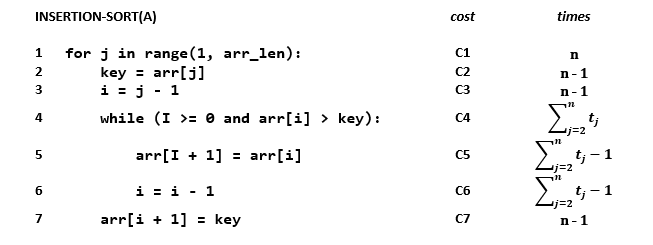
\includegraphics[scale=0.7]{fig/InsertionSortAnalysis.png}%
	\caption{Analisis \textit{Insertion Sort}}%
	\label{fig:analisis-insertion-sort}%
\end{figure}

\FloatBarrier

Penjelasan lebih detil dari Gambar \ref{fig:analisis-insertion-sort} adalah sebagai berikut.

\begin{enumerate}
	\item Baris 1: Memiliki biaya sebesar $c_1$ dimana biaya tersebut akan diulang sebesar $n$ kali. Pengulangan sebesar $n$ kali dikarenakan adanya sebuah looping ``for i in range(1, arr\_len)''. Looping \textbf{for} akan dieksekusi oleh komputer sebanyak arr\_len kali. Untuk mempermudah perhitungan maka kita lambangkan arr\_len sebagai $n$. Sebagai contohnya, jika arr\_len bernilai 5, maka baris 1 akan diulang sebanyak 6 kali (1,2,3,4 dan 5 bernilai $True$ dan 1 kali terakhir bernilai $False$) atau dengan kata lain $n$ bernilai 6.
	\item Baris 2 -- 3: Memiliki biaya masing-masing $c_{2}$ dan $c_{3}$. Kedua baris ini masing-masing diulang sebanyak $n-1$ kali. Kenapa $n-1$ kali? Karena semua baris di dalam \textit{looping} \textbf{for} hanya diulang untuk setiap \textbf{for} yang bernilai $True$.
	\item Baris 4: Baris ini diulang sebanyak $\sum\limits_{j=2}^n t_{j}$ kali. Di baris ini ada dua buah \textit{looping}: \textit{outer loop} -- \textbf{for} dan \textit{inner loop} -- \textbf{while}. Untuk \textit{inner loop} dilambangkan dengan $t_{j}$. $t_{j}$ melambangkan jumlah \textit{looping inner loop}. Ketika \textit{inner loop} dan \textit{outer loop} digabungkan maka menjadi $\sum\limits_{j=2}^n t_{j}$.  
\end{enumerate}                                       
                                     
Total waktu eksekusi dari Algoritma \ref{algo:insertion} dilambangkan dengan $T(n)$ dimana:

\begin{equation}\label{eq:eksekusi-insertion-1}
    T(n) = c_{1}n + c_{2}(n-1) + c_{4}(n-1) + c_{5}\sum\limits_{j=2}^n t_{j} + c_{6}\sum\limits_{j=2}^n (t_{j}-1) + c_{7}\sum\limits_{j=2}^n (t_{j}-1) + c_{8}(n-1) 
\end{equation} 

Dari Persamaan \ref{eq:eksekusi-insertion-1}, kita bisa menghitung total waktu eksekusi ($T(n)$) yang bergantung kepada variabel $n$ atau banyaknya bilangan masukan. Semakin banyak bilangan masukan maka $T(n)$ akan semakin tinggi dan sebaliknya. Akan tetapi, $T(n)$ tidak hanya bergantung pada banyaknya bilangan masukan, tetapi bergantung juga kepada susunan bilangan tersebut. Bagaimana jika \textit{array} bilangan tersebut sudah terurut? Bukankah waktu yang dibutuhkan akan lebih sedikit dibandingkan jika semua bilangan tersebut terbalik urutannya?

Seandainya semua bilangan sudah terurut maka baris ke 5 dan baris ke 6 dari Algoritma \ref{algo:insertion} tidak perlu dijalankan lagi karena perintah di baris ke 4 akan selalu menghasilkan $False$. Dengan kata lain nilai dari $t_{j}$ akan selalu konstan yaitu 1. Maka Persamaan \ref{eq:eksekusi-insertion-1} akan menjadi sebagai berikut:

\begin{equation}\label{eq:insertion-sort-optimal}
    \begin{aligned}
        T(n) & = c_{1}n + c_2(n-1)+c_4(n-1)+c_5(n-1)+c_8(n-1) \\
             & = (c_1+c_2+c_4+c_5+c_8)n-(c_2+c_4+c_5+c_8)
    \end{aligned}
\end{equation}

Persamaan \ref{eq:insertion-sort-optimal} merupakan apa yang biasa disebut sebagai \textit{best case} atau kasus terbaik. Jika persamaan tersebut disederhanakan maka bisa ditulis sebagai $an+b$ atau yang biasa disebut sebagai fungsi linear akan $n$. 

Untuk kasus terburuk (\textit{worst case}) akan terjadi jika \textit{array} angka yang akan diurut disusun secara terbalik semua (misalnya mengurut bilangan $\left\{5,4,3,2,1\right\}$ menjadi $\left\{1,2,3,4,5\right\}$). Untuk kasus tersebut, berarti kita harus mencocokkan setiap angka di \textit{inner loop}, atau dengan kata lain nilai dari $t_{j}$ adalah sama dengan nilai dari $j$ yang berasal dari \textit{outer loop}. 

\begin{equation}\label{eq:eksekusi-insertion-sort-2}
    \begin{aligned}
        T(n) & = c_1n + c_2(n-1) + c_4(n-1) + c_5(\frac{n(n+1)}{2}-1) + c_6(\frac{n(n-1)}{2}) \\ 
             &   + c_7(\frac{n(n-1)}{2})+c_8(n-1) \\
             & = (\frac{c_5}{2}+\frac{c_6}{2}+\frac{c_7}{2})n^2+(c_1+c_2+c_4+\frac{c_5}{2}-\frac{c_6}{2}-\frac{c_7}{2}+c_8)n \\
             &   -(c_2+c_4+c_5+c8)
    \end{aligned}
\end{equation}

Persamaan \ref{eq:eksekusi-insertion-sort-2} bisa disederhanakan menjadi $an^2+bn+c$ atau yang disebut juga dengan fungsi kuadratic akan $n$. 

Dari persamaan \ref{eq:eksekusi-insertion-sort-2} yaitu $an^2+bn+c$, terdapat tiga konstan ($a$, $b$, dan $c$) yang besarnya tergantung pada $c_i$. Untuk membuat lebih sederhana, kita bisa membuat abstraksi yang lebih sederhana yaitu dengan hanya memperhatikan laju pertumbuhan fungsi (\textit{order of growth}). Untuk itu kita cukup hanya perlu memperhatikan order tertinggi dari fungsi yaitu $an^2$ karena order yang lebih rendah lajut pertumbuhannya tidak begitu signifikan untuk nilai $n$ yang besar. Untuk itu kita tulis bahwa \textit{insertion sort} memiliki \textit{worst case} $O(n^2)$.

